\subsection{1018MS Corrosion Parameters from Anodic/Cathodic Sweeps}




\begin{table}[h!]
	\centering
	\begin{tabular}{lllrrrr}
\toprule
  &     &     &  $A_{\text{H}}$ (V) &  $A_{\text{Fe}}$ (V) &  $j_{\text{corr}}$ (A/mm$^2$) &  $\Delta \phi_{\text{corr}}$ (V) \\
Scan & Soln & Dir &                     &                      &                               &                                  \\
\midrule
0 & H$_2$SO$_4$ & Asc &          -8.778e-02 &            8.903e-02 &                     1.784e-06 &                       -4.794e-01 \\
  &     & Des &          -9.588e-02 &            8.833e-02 &                     1.888e-06 &                       -4.843e-01 \\
2 & H$_2$SO$_4$ & Asc &          -8.341e-02 &            8.519e-02 &                     1.663e-06 &                       -4.730e-01 \\
  &     & Des &          -5.730e-02 &            8.076e-02 &                     3.096e-06 &                       -4.842e-01 \\
4 & HCl & Asc &          -7.706e-02 &            8.553e-02 &                     1.277e-06 &                       -5.022e-01 \\
  &     & Des &          -9.978e-02 &            8.326e-02 &                     1.765e-06 &                       -5.090e-01 \\
6 & HCl & Asc &          -7.490e-02 &            9.225e-02 &                     1.469e-06 &                       -4.806e-01 \\
  &     & Des &          -1.035e-01 &            8.415e-02 &                     2.140e-06 &                       -5.097e-01 \\
\bottomrule
\end{tabular}

\end{table}

\begin{table}[h!]
	\centering
	\begin{tabular}{lllrrrrr}
\toprule
  &     &     &  $\sigma^2(A_{\text{H}})$ &  $\sigma^2(A_{\text{Fe}})$ &  $\sigma^2(j_{\text{corr}})$ &  $\sigma^2(\Delta \phi_{\text{corr}})$ &   n \\
Scan & Soln & Dir &                           &                            &                              &                                        &     \\
\midrule
0 & H$_2$SO$_4$ & Asc &                 2.424e+02 &                  2.786e+02 &                    2.343e-15 &                              1.401e-09 &  95 \\
  &     & Des &                 9.089e+00 &                  1.206e+01 &                    6.030e-15 &                              3.785e-09 &  95 \\
2 & H$_2$SO$_4$ & Asc &                 9.356e-06 &                  1.890e-05 &                    1.091e-13 &                              3.618e-08 &  96 \\
  &     & Des &                 4.672e+00 &                  8.336e+00 &                    1.320e-14 &                              7.072e-09 &  96 \\
4 & HCl & Asc &                 3.771e+01 &                  4.110e+01 &                    1.809e-15 &                              3.614e-09 &  97 \\
  &     & Des &                 1.705e+03 &                  1.066e+03 &                    1.665e-15 &                              7.201e-10 &  97 \\
6 & HCl & Asc &                 4.333e+02 &                  2.297e+02 &                    1.349e-15 &                              1.066e-09 &  97 \\
  &     & Des &                 3.935e+03 &                  8.564e+03 &                    1.584e-15 &                              2.366e-10 &  97 \\
\bottomrule
\end{tabular}

\end{table}

\begin{figure}[h!]
	\centering
	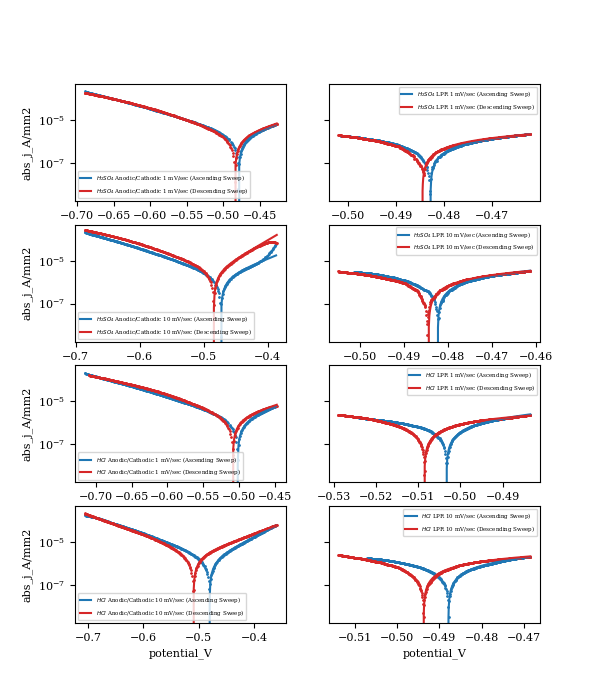
\includegraphics[width=1.0\linewidth]{resources/fig_2b.png}
\end{figure}


\subsection{1018MS Corrosion Parameters from LPR Sweeps}

\begin{table}[h!]
	\centering
	\begin{tabular}{llllrrrr}
\toprule
  &     &           &     &  $j_{corr}$ (A/mm$^2$) &  $\Delta \phi_{corr}$ (V) &  $\sigma^2(j_{corr})$ &    n \\
Scan & Soln & Rate & Dir &                        &                           &                       &      \\
\midrule
1 & H$_2$SO$_4$ & 1 mV/sec & Asc &              1.342e-06 &                -4.830e-01 &             6.559e-16 &  338 \\
  &     &           & Des &              1.354e-06 &                -4.841e-01 &             3.434e-15 &  421 \\
3 & H$_2$SO$_4$ & 10 mV/sec & Asc &              2.058e-06 &                -4.822e-01 &             2.552e-15 &  342 \\
  &     &           & Des &              1.941e-06 &                -4.849e-01 &             1.070e-14 &  444 \\
5 & HCl & 1 mV/sec & Asc &              1.302e-06 &                -5.032e-01 &             4.275e-14 &  353 \\
  &     &           & Des &              1.335e-06 &                -5.085e-01 &             2.300e-14 &  442 \\
7 & HCl & 10 mV/sec & Asc &              1.265e-06 &                -4.879e-01 &             4.494e-15 &  342 \\
  &     &           & Des &              1.297e-06 &                -4.937e-01 &             2.720e-14 &  443 \\
\bottomrule
\end{tabular}

\end{table}

\begin{figure}[h!]
	\centering
	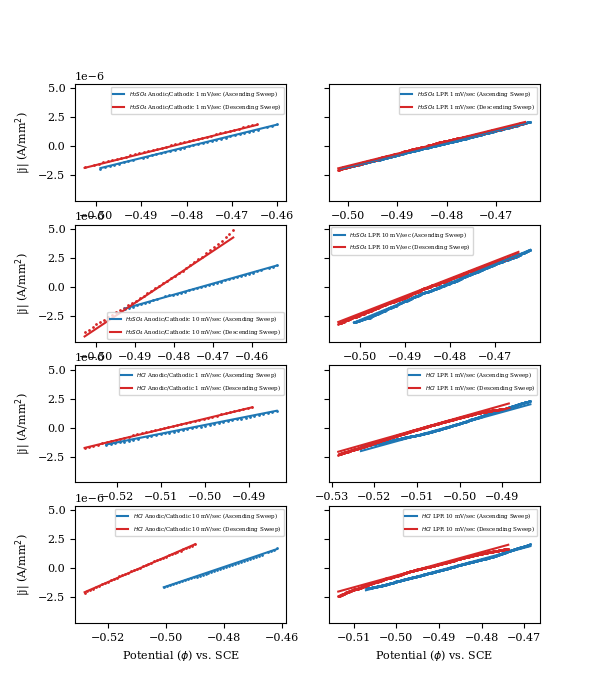
\includegraphics[width=1.0\linewidth]{resources/fig_2c.png}
\end{figure}

\subsection{Deconvolution of 304SS Polarization Sweeps}


\begin{table}[h!]
	\centering
	\begin{tabular}{lrrrr}
\toprule
{} &  $\phi_0$ (V) &  $j_0$ (A/mm$^2$) &    $A$ (V) &  $\rho_{\text{lim}}$ ($\Omega \cdot$mm) \\
Reaction                             &               &                   &            &                                         \\
\midrule
H$^+$ reduction                      &    -3.728e-01 &        -9.612e-08 & -1.138e-01 &                               1.587e+02 \\
Fe oxidation (passivation-limited)   &    -3.927e-01 &         7.891e-07 &  3.505e-03 &                               3.905e+04 \\
Cr$_2$O$_3$ barrier breakdown (asc)  &     9.688e-01 &         9.902e-07 &  3.701e-02 &                               1.968e+03 \\
H$_2$O breakdown (asc)               &     1.596e+00 &         1.065e-04 &  2.025e-01 &                              3.230e-312 \\
unknown reduction reaction           &     1.500e-01 &        -5.000e-11 & -3.289e-02 &                               2.000e+05 \\
Cr$_2$O$_3$ solution deposition      &     1.070e+00 &       -1.812e+169 & -9.784e-06 &                               4.502e+06 \\
Cr$_2$O$_3$ barrier breakdown (desc) &     9.814e-01 &         4.565e-07 &  5.713e-02 &                               1.324e+03 \\
H$_2$O breakdown (desc)              &     1.599e+00 &         1.016e-04 &  1.971e-01 &                               3.765e-06 \\
\bottomrule
\end{tabular}

\end{table}

\begin{table}[h!]
	\centering
	\begin{tabular}{lrrr}
\toprule
{} &  $\phi_{pass}$ (V) &  $\alpha_{pass}$ (V$^{-3}$) &  $\rho_{pass}$ ($\Omega \cdot$mm) \\
Reaction                             &                    &                             &                                   \\
\midrule
Fe oxidation (passivation-limited)   &         -3.530e-01 &                   4.814e+00 &                         6.966e+06 \\
Cr$_2$O$_3$ barrier breakdown (asc)  &          1.300e+00 &                   8.971e-03 &                         5.670e+07 \\
unknown reduction reaction           &         -3.000e-02 &                   1.000e+01 &                         1.000e+07 \\
Cr$_2$O$_3$ barrier breakdown (desc) &          1.239e+00 &                   7.470e-03 &                         2.868e+07 \\
\bottomrule
\end{tabular}

\end{table}

\begin{figure}[h!]
	\centering
	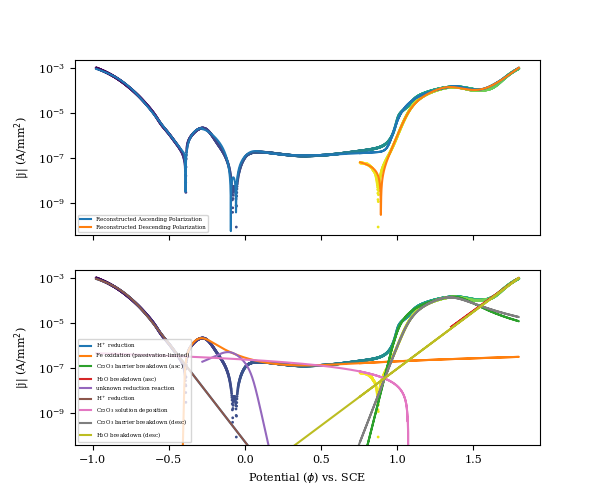
\includegraphics[width=1.0\linewidth]{resources/fig_2a1.png}
\end{figure}

\begin{table}[h!]
	\centering
	\begin{tabular}{lrrrr}
\toprule
{} &  $\phi_0$ (V) &  $j_0$ (A/mm$^2$) &    $A$ (V) &  $\rho_{lim}$ ($\Omega \cdot$mm) \\
Reaction                           &               &                   &            &                                  \\
\midrule
H$^+$ reduction                    &    -3.478e-01 &        -3.793e-07 & -1.145e-01 &                        3.210e+02 \\
Fe oxidation (diffusion-limited)   &    -4.695e-01 &         1.498e-08 &  3.570e-02 &                        2.157e+03 \\
Fe oxidation (passivation-limited) &    -4.695e-01 &         1.498e-08 &  3.570e-02 &                        2.157e+03 \\
Cl$^-$ ion pitting                 &     3.928e-01 &         8.802e-05 &  4.837e-02 &                        9.837e+01 \\
\bottomrule
\end{tabular}

\end{table}

\begin{table}[h!]
	\centering
	\begin{tabular}{lrrr}
\toprule
{} &  $\phi_{pass}$ (V) &  $\alpha_{pass}$ (V$^{-3}$) &  $\rho_{pass}$ ($\Omega \cdot$mm) \\
Reaction                           &                    &                             &                                   \\
\midrule
Fe oxidation (passivation-limited) &         -1.643e-01 &                   5.187e+03 &                         5.946e+03 \\
\bottomrule
\end{tabular}

\end{table}

\begin{figure}[h!]
	\centering
	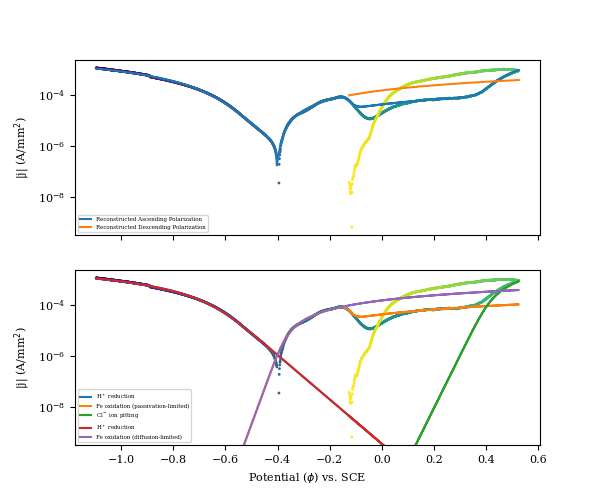
\includegraphics[width=1.0\linewidth]{resources/fig_2a2.png}
\end{figure}


